\chapter{Towards an evaluation platform for inductive model synthesis\label{chapter:stamina}}

As discussed in chapter~\ref{chapter:evaluation}, an induction algorithm is commonly evaluated by reporting an accuracy measure of the model it learns for increasing size of a training sample. Plots typically illustrates the convergence towards a ``good'' model when the training sample becomes rich enough. Practical evaluations have been conducted on RPNI as well as numerous of its variants in \cite{Lang98,Damas06,Dupont08,Lambeau08}. In that respect, the Abbadingo contest~\cite{Lang98} have had a notable impact, first because it provides a reusable evaluation protocol and benchmarks for induction algorithms and second, because it helped discovering the evidence-driven state merging heuristic used by Blue-Fringe, on which QSM itself relies. 

Abbadingo focussed on learning DFAs from positive and negative strings along two difficulty dimensions, the size of the automaton to learn and the sparsity of the training sample. All other parameters were fixed, notably the alphabet size which was equal to 2 for all problems (other candidate parameters include the ratio of final states over non-final ones, the density and depth of the automaton, the ratio of positive over negative strings in the training sample, the distribution of string lengths, and so on).

Fixing parameters of benchmarks and contests helps keeping competition objectives sufficiently clear and understandable for users. If also makes sound analysis results easier to obtain, due to the presence of only a few degrees of freedom. On the other hand, fixing parameter values has an important impact because it limits the applicability of the conclusions drawn as well as their generalization. In that respect, the conclusions drawn in the previous chapter all rely on an -- sometimes implicit -- assumption of an alphabet of 2 letters. While extrapolating results to larger alphabets appears natural, it must be done with care.

Our use of the Abbadingo protocol was initially motivated by the necessity to compare our results with previous ones of grammatical inference. Unfortunately, restricting our attention to binary alphabets is arguable from a software engineering point of view, for two reasons. First because behavior models are often defined on 30 events or more. Second, and probably more important, because using binary alphabets has a strong influence on the class of automata considered. Therefore, one can certainly question the representativeness of synthetic machines and samples used in the previous chapter for capturing certain characteristics of behavior models. 

This overal questioning of the influence of the alphabet size on the synthesis performance motivated the Stamina competition (Stamina stands for \emph{State Machine Inference Approaches}) that we ran between march and december 2010 in collaboration with the universities of Sheffield and Leicester, and officially sponsored by the Engineering and Physical Sciences Research Council\footnote{http://www.epsrc.ac.uk/}. Its aim was to identify the best technique to infer state machines presenting characteristics of behavior models while focussing on the complexity of the learning with respect to the alphabet size, an aspect that has not been tackled in previous competitions or benchmarks. For this, Stamina extends Abbadingo -- with which it shares certain features -- but relies on adapted protocols for generating target machines and samples, among other differences. 

The winning algorithm DFASAT -- as well as a few additional competitors -- significally outperformed the baseline (Blue-fringe) on a variety of problems. This technique mixes SAT solving and state merging and uses a new scoring heuristic that proved useful to tackle the learning task in presence of alphabets of more than two letters. In addition to pushing forward the state of the art of the induction problem, the competition triggered interest from at least three communities, namely Machine Learning, Software Engineering and Formal Methods. The Stamina website\footnote{http://stamina.chefbe.net/} is still available and has been slightly updated to serve as an online benchmark and evaluation platform for model synthesis, instead of a formal competition.

This chapter is organized as follows. Section~\ref{section:stamina-background} provides background on the Abbadingo competition and discusses the weaknesses of its protocol when considering behavior models. The detailed setup of the Stamina competition is explained in section~\ref{section:stamina-setup}. The main results of the competition are then summarized in section~\ref{section:stamina-results}, including a short description of the winning technique. Section~\ref{section:stamina-platform} closes this chapter with a description of the changes made to convert the competition server to an evaluation platform and summarizes future work along this direction.

\section{From Abbadingo to Stamina\label{section:stamina-background}}

\subsection{Background on Abbadingo}

The Abbadingo competition has been designed as a grid of 16 induction problems. The general principle of learning applies: the learner is provided a set of training strings labeled as positive or negative by an unseen DFA and is required to predict the labels that the DFA would assign to a set of testing strings. The 16 problems formed a grid of two difficulty dimensions. The first dimension is the size of the target automata, as the number of its states (64, 128, 256 and 512 states were considered). The second dimension is the sparsity of the training sample. Four sparsity levels were considered, with the exact number of strings -- a few thousands -- increasing also with the automaton size considered. The exact size of each training sample has been tuned by manually inspecting learning curves of the Trakhenbrot-Barzdin algorithm, considered as one of the state-of-the-art induction algorithm in 1997. The problem grid was adjusted in such a way that the latter algorithm solved the four problems with largest samples.

In Abbadingo, the target automata, training and test strings were all drawn from uniform random distributions. Random automata were generated by constructing and minimizing degree-2 directed graphs (for recall, only alphabet of two letters were considered), with the label of edges (the letter) and states (final or not) being choosen by flipping a fair coin. To keep the generation of the training set sufficiently simple, only automata of depth of exactly $2log_2(n)-2$ were considered for the problem grid. A training set for a target of size $n$ was made of a random sample drawn without replacement from a uniform distribution over the collection of $16n^2 -1$ binary strings whose length lies between 0 and $2log_2(n)+3$ inclusively. This latter bound was chosen to have a good chance of reaching the deepest state of the automaton, a necessary criteria towards a structurally complete sample, which was not guaranteed though. The testing set consisted in 1800 strings drawn from the remaining strings and, as a consequence, did not overlap with the training set.

The testing protocol of Abbadingo consisted in the learner labeling each string of the test set and submitting these labelings to a testing oracle available online\footnote{the server is now hosted at http://abbadingo.cs.nuim.ie/}. To avoid hill climbing -- where the feedback of the competition server could be used by the learner to iteratively optimize a first solution -- this oracle only provided a 1 bit of feedback which told whether or not the accuracy (the ratio of the number of strings correctly labeled over the total number of test strings, i.e. 1800) of the labeling was at least 99\%. In that case, the problem was considered solved and the participant gained credit for it provided that she was the first to break it. Abbadingo actually allowed multiple winners by defining a partial order of problem difficulty: a problem $A$ was harder than a problem $B$ if its DFA had more states \emph{and} its training sample was sparser. 

Two winners, Rodney Price and Hugues Julli\'e, won the competition with similar algorithms relying on what has since been called \emph{evidence driven state merging} (EDSM). This term captures the strategy of first performing state merges that are supported by the most evidence. Among other contributions, the competition has helped finding a good scoring heuristics based on the number of final states merged. Also, mixing this evidence driven idea with the red-blue merge order described previously (see chapter~\ref{chapter:inductive-synthesis}) leads to the particularly fast and simple algorithm known as \emph{Blue-fringe}, for which Abbadingo provided a reference description~\cite{Lang98}.

\subsection{Inadequacies for software behavior models}

Since the end of the competition, Abbadingo has turned to a reusable protocol (and benchmark) for induction techniques. To situate and compare our results, the evaluations proposed in chapter~\ref{chapter:inductive-synthesis} of the present thesis have been precisely conducted on that protocol. However, as already stated, the fact that Abbadingo fixed the size of the alphabet to only two letters limits the relevance of reusing its protocol for evaluating behavior model synthesis techniques. This is mainly because behavior models are commonly defined on larger sets of events. As an example, the small phone case-study of section~\ref{section:evaluation-re} already uses 16 distinct events for a state machine of only 23 states. Moreover, considering binary alphabets only has deeper consequences than one would expect at first glance:

\begin{description}
\item[Automata] The automata randomly generated by Abbadingo have a quasi-constant state degree (number of indident edges). This is a consequence of using binary alphabets: due to the its deterministic nature, an automaton of $n$ states has at least $n$ and at most $2n$ edges, randomly distributed between its states. 

In contrast, automata modeling software systems involve transitions that may be triggered by any of a large number of events (mouse clicks, function names IO events, etc.). The number of outgoing transitions for a given state can be very large and vary significantly from state to state. A review of the state machines found in the litterature shows that while most states have in- and out-degrees of one or two transitions, state machines tend to contain a small proportion of states with a high in-degree (e.g. modeling exception handling, typically) or a high out-degree (an \emph{idle} software agent waiting for external stimuli in terms of input events). Other states are \emph{sink} accepting states, that is, they have an out-degree of 0 (explicit modeling of the ability of a system to halt). And so on.

The automata generated by by Abbadingo do not present such characteristics, due to the small alphabet size. Moreover, the random generation procedure -- because of the uniform edge distribution it implies -- would not naturally lead to automata presenting such characteristics, even if adapted to consider larger alphabets.

\item[Samples] Samples in Abbadingo are simply drawn from uniform random distribution over the collection of all (binary) strings up to a prescribed length. The target machine was then used to classify these strings as positive or negative. For statistical reasons, this procedure leads to samples that are naturally balanced with respect to those positive vs. negative labels. 

Unfortunately, this procedure is no longer viable when considering larger alphabets (unless state machines present similar characteristics to the ones of Abbadingo, which is not the case, as previously discussed). The main reason is that an overwhelming majority of random sequences in $\Sigma^*$ is likely to be classified as negative. The few positive strings that would be made available is unlikely to provide a useful coverage of the target machine.

\item[Scoring] The choice of the accuracy measure (defined in Abbadingo as the proportion of test strings that are correctly classified by the automaton learned) is also arguable if one relaxes the assumption of having balanced test samples~\cite{Walkinshaw2008}. In the extreme case of a test set largely overwhelmed by negative strings for example, a learner classifying all strings as negative would obtain a confortable score.
\end{description}

As shown, conducting evaluations while overcoming the usage of binary alphabets implies rethinking important parts of the underlying protocol. To capitalize over and share the cost of such a work, it took the form of launching the Stamina competition, whose setup is now described in more details.

%%%%%%

\section{Setup of Stamina\label{section:stamina-setup}}

The competition scenario chosen for Stamina is very similar to the one of Abbadingo: 

\begin{quotation}
A learner downloads a training set made of positive and negative strings, infers a model using her induction technique, uses it to label strings of a test sample and finally, submits this labeling to the competition server. The latter scores the submission and provides a binary feedback, according to whether the problem is considered broken or not.
\end{quotation}

If the competition scenario is similar, Stamina differs from Abbadingo in that it focusses on the complexity of the learning with respect to the alphabet size, and therefore relies on an adapted generation protocol for target automata and samples. The next sections details the choices that have been made and the key differences with Abbadingo.

\subsection{Competition grid}

As in Abbadingo, induction problems are classified in a grid. Here, the competition grid is divided in cells of five problems each, where each cell corresponds to a particular combination of sparsity and alphabet size. Table~\ref{stamina:table:problem-grid} shows how problems are distributed in cells. Easier problems (with a smaller alphabet and a larger sample) are towards the upper-left of the table, and the harder problems (larger alphabet and smaller sample) are towards the bottom-right.

\begin{table}[h]
\begin{center}
\begin{tabular}{c|c c c c}
&\multicolumn{4}{|c}{Sparsity}\\ 
\textbf{$|\Sigma|$} & \textbf{100\%} & \textbf{50\%} & \textbf{25\%} & \textbf{12.5\%}\\
\hline
\textbf{2}  & 1-5   & 6-10  & 11-15 & 16-20 \\
\textbf{5}  & 21-25 & 26-30 & 31-35 & 36-40 \\
\textbf{10} & 41-45 & 46-50 & 51-55 & 56-60 \\
\textbf{20} & 61-65 & 66-70 & 71-75 & 76-80 \\
\textbf{50} & 81-85 & 86-90 & 91-95 & 96-100\\
\end{tabular}
\end{center}
\caption{\label{stamina:table:problem-grid}Grid of 100 problems distributing the induction difficulty among two dimensions: sparsity of the learning sample and alphabet size.}
\end{table}

\noindent The key differences and similarities with Abbadingo are:

\begin{itemize}

\item An increasing size of the alphabet forms a first difficulty dimension, ranging from 2 to 50 letters. The lower bound allows comparing results with Abbadingo on easiest problems while the upper bound is representative of behavior models found in the litterature.

\item Unlike Abbadingo in which the varying automaton size is a difficulty dimension (ranging from 64 to 512), Stamina only considers automata of roughly 50 states. However, these automata present characteristics of behavior models, in terms of the variance of their state degree, among others (see section~\ref{subsection:stamina-machines})

\item The second difficulty dimension, namely a decreasing size of the training sample, is shared with Abbadingo. However, samples in Stamina are generated ``from the machine'' by a random walk procedure, instaed of randomly drawn from all possible strings (see section~\ref{subsection:stamina-samples}).

\item In Stamina, each cell contains five similar problems and is given a difficulty level according to the average score obtained by Blue-fringe on the problems it contains (see section~\ref{subsection:stamina-baseline}). An implementation of this baseline algorithm was made available for download during the competition.

\item Instead of an accuracy measure, submissions were scored using a \emph{binary classification rate} (BCR) because it places an equal emphasis on the accuracy of an inferred model in terms of its acceptance of positive sequences, as well as its rejection of sequences that should be rejected. A threshold of 99\% is required to consider a problem broken. A cell is broken if its five problems are broken by the same participant.

\item The winner of the competition was the first technique to solve a hardest cell (in terms of the difficulty level aformentioned), among those solved in the competition. This contrasts with Abbadingo as it implies the existence of only one winner.

\end{itemize}

\subsection{State Machines\label{subsection:stamina-machines}}

In order to generate state machines representative of the ones encountered in the software engineering community, a quick review of software models has been conducted. Observations have been made on a small sample (about 20 systems) of case-study models found in research publications. State machine models were analyzed in terms of their states, transitions, alphabet sizes, in-/out degree and depth. Although the sample is too small to form any authoritative conclusions, findings can be interpreted as being indicative. Following these observations, the target machines used in the competition have been generated using a variant of the Forest-Fire algorithm~\cite{Leskovec2007}. The algorithm has been tuned to generate state machines presenting the following characteristics:

\begin{description}

\item[Number of states] All state machines have approximately 50 states. Although somewhat larger than the conventional state machines identified in the literature, this is to ensure that any techniques submitted to this competition could scale to infer models for reasonably complex software systems. Also, is has been decided not to consider state machines of exactly 50 states to avoid having a very strong bias in the competition. Automaton sizes actually range from 41 to 59 states, even if this information was not disclosed as such during the competition.

\item[Accepting ratio] A roughly equal proportion of accepting and rejecting states has been chosen, a feature is shared with Abbadingo. While most software models, and LTS in particular, have all accepting states it has been decided to keep non accepting states as well. Doing so keeps the competition sufficiently close to former regular induction setups, and avoids restricting it to the inference of prefix-closed regular languages in particular. As already discussed in chapter~\ref{chapter:inductive-synthesis}, infering prefix-closed languages looks an easier problem than general regular inference. Hence, a competition winner would be expected to perform equaly well, if not better, when infering machines with all accepting states.

\item[Degree distribution] Following observations from the litterature, state machines present an important variance of their state degree, especially on largest alphabets. Also, they may have sink accepting states, i.e. with no outgoing transition.

\item[Deterministic and minimal] Following common setup of regular inference experiments, the machines considered in the competition are both deterministic and minimal.

\end{description}

\subsection{Training and test samples\label{subsection:stamina-samples}}

Training and test samples have been generated using a dedicated generation procedure. This procedure aims at simulating the way examples of system behaviour are usually obtained in the software engineering community (a collection of program traces at an implementation level or the generation of scenarios at a design level, for instance). Samples generated present the following characteristics:

\begin{description}

\item[Generated by the target] Positive strings have been generated by randomly walking the target machines. A dedicated algorithm generates positive strings by walking through the automaton from the initial state, randomly selecting outgoing transitions with a uniform distribution. When an accepting state v is reached, the generation ends with a probability of $1.0/(1 + 2*outdegree(v))$. This procedure simulates an ``end of string'' transition from state $v$ with half the probability of an existing transition. The length distribution of the strings generated is approximately centered on $5 + depth(automaton)$. As in Abbadingo, this provides a good chance to reach the deepest state of the automaton, even if no guarantee was given of having a structurally complete sample.

\item[Negative strings] Negative strings are generated by randomly perturbing positive strings generated as above. Three kinds of edit operation are considered: substituting, inserting, or deleting a symbol. The editing position is randomly chosen according to an uniform distribution over the string length. Substitution and insertion also use an uniform distribution over the alphabet. The number of editing operations is chosen according to a Poisson distribution (with a mean of 3) and the three editing operations have an equal change of being selected. The randomly edited string is included in the negative sample provided it is indeed rejected by the target machine. Otherwise, it is simply discarded.

\end{description}

The random walk algorithm and perturbation procedure serve as building blocks for the generation of training and test samples for each problem. Using them, a set of 20.000 strings is first sampled from the target machine. This sample contains roughly equal number of positive and negative strings and usually contains duplicates. The distinct strings of the initial sample are then equally partitioned into two sets, taking care of respecting the positive and negative balance in each one. The first set is used to generate the test sample, the second one to generate the learning sample. The test sample contains 1,500 strings randomly drawn without replacement from the first set. The test set neither contains duplicates (to avoid favoring repeated strings in the scoring metric), nor intersects with the training set. The official training sets are sampled from the second set with different levels of sparsity (100\%, 50\%, 25\%, 12.5\%) and usually contain duplicates, as a consequence of the random walk generation from the target machine. As a consequence of this procedure, training and test sets do not intersect.

\subsection{Blue-fringe baseline\label{subsection:stamina-baseline}}

Blue-fringe has been ran on all problems of the grid with the main objective of adjusting the grid to guarantee the feasibility of the competition. Similarly to Abbadingo, the idea is to adjust free parameters (actual sizes of the training and test sets, average length of the strings with respect to the automaton depth, and so on) in such a way that the state of the art algorithm breaks the easiest problems. This trial-and-error process converged with three problems broken in the easiest cell (therefore not itself broken) and reasonnable scores for the two remaining problems as well as  immediately adjacent cells. 

The performance of the baseline are summarized in Table~\ref{table:stamina-baseline} and illustrated with convergence curves in Figure~\ref{stamina:image:bluefringe-performance}. As shown, the BCR score decreases along each of the difficulty dimensions, experimentally confirming the expected effect of an increasing alphabet size on the indution difficulty. Using these scores, the difficulty level of each cell has been calibrated using the rules defined in Table~\ref{stamina:table:calibration}.

\begin{table}
\begin{center}
\begin{tabular}{c|c c c c}
&\multicolumn{4}{|c}{\textbf{Sparsity}}\\ 
\textbf{$|\Sigma|$} & \textbf{100\%} & \textbf{50\%} & \textbf{25\%} & \textbf{12.5\%}\\
\hline
\textbf{2}  & 0.99 (1) & 0.95 (1) & 0.67 (3) & 0.66 (3)\\
\textbf{5}  & 0.97 (1) & 0.78 (2) & 0.59 (4) & 0.52 (4)\\
\textbf{10} & 0.93 (1) & 0.64 (3) & 0.51 (4) & 0.50 (4)\\
\textbf{20} & 0.91 (1) & 0.63 (3) & 0.54 (4) & 0.51 (4)\\
\textbf{50} & 0.81 (2) & 0.64 (3) & 0.57 (4) & 0.50 (4)\\
\end{tabular}
\end{center}
\caption{Average BCR of Blue-fringe in each cell; the difficulty level is shown in parentheses.\label{table:stamina-baseline}}
\end{table}

\begin{figure}
\centering\scalebox{.4}{
  \includegraphics*{src/6-stamina/images/bluefringe-performance}}
  \caption{Performance curves of Blue-fringe\label{stamina:image:bluefringe-performance}.}
\end{figure}

\begin{table}
\begin{center}
\begin{tabular}{c|c}
Difficulty level & Score\\
\hline
1&$0.9 \leq score \leq 1$\\
2&$0.7 \leq score < 0.9$\\
3&$0.6 \leq score < 0.7$\\
4&$0 \leq score < 0.6$\\
\end{tabular}
\end{center}
\caption{\label{stamina:table:calibration}Calibrating cell difficulties, based on the scores given in Table~\ref{table:stamina-baseline}}
\end{table}

\subsection{Submission and Scoring}

As in Abbadingo, solutions in Stamina had to be submitted as a binary string to the competition server. For this, the competitor was expected to produce a binary sequence of labels where, for each test string, a 1 is added to the sequence if the string is considered to be accepted, and a 0 otherwise. To establish the accuracy, such a sequence is compared to a reference string representing the correct classifications of the test set on the target model. The overlap between the two binary strings is measured with the \emph{Balanced Classification Rate (BCR)}. The Harmonic BCR measure is chosen because it places an equal emphasis on the accuracy of an inferred model in terms of its acceptance of positive sequences, as well as its rejection of sequences that should be rejected. It also does not require the test set to be balanced in terms of its positive / negative sequences~\cite{Walkinshaw2008}. 

Harmonic BCR is the harmonic mean of two factors. $Sensitivity$ is the proportion of positive matches that are predicted to be positive and $Specificity$ is the proportion of true negatives that are predicted to be negative. So in terms of the sets true positives ($TP$) and false positives ($FP$), 

$$Sensitivity=\frac{|TP|}{|TP \cup FN|}$$ 

$$Specificity=\frac{|TN|}{|TN \cup FP|}$$

$$BCR=\frac{2*Sensitivity*Specificity}{Sensitivity + Specificity}$$

Note that conventionally, BCR is simply computed as the arithmetic mean of sensitivity and specificity, but the harmonic mean has been preferred because it favours balance between the two.

As in Abbadingo, hill-climbing is made impossible by the competition server only responding to a submission with a binary answer according to whether the problem is broken or not. For recall, a problem is considered broken if the BCR score obtained is greater than or equal to 0.99. A cell is considered broken if all of its 5 problems are broken. A section dedicated to each participant has been implemented on the website to provide visual feedback about the performance of their algorithm(s). In this section, problems and cells of a personal problem grid turn to green when broken.

%%%%%%

\section{Competition results\label{section:stamina-results}}

The competition has been started on March 2010, the 31th of December being announced as an official deadline for submitting results. Between these two dates, 1856 submissions were made by 11 challengers. Among these submissions, 61 reached a BCR score of at least 99\%, breaking 42 different problems in 10 different cells.

The competition hall of fame is shown in Fig.\ref{stamina:table:hall-of-fame}. The easiest cell (alphabet 2, sparsity 100\%) was quickly broken --~five days after the competition start~-- by Manuel V\'azquez de Parga Andrade with the Equipo algorithm (learning of automata teams, see~\cite{Garcia:2010}). This first result has been followed by an apparent lull in the competition. Some challengers were actually submitting at that time but without successfully breaking new problems and cells so that this activity was not directly visible on the competition website. A few weeks after, Marijn Heule and Sicco Verwer, with the DFASAT algorithm~\cite{Heule10}, started solving all cells of difficulty~1 in the left-most column. After a new small lull, they eventually broke the first cell of difficulty 2 (alphabet 50, sparsity 100\%) therefore taking the head of the competition. They eventually won the competition with an extra cell being broken (alphabet 50, sparsity 50\%), the only cell of difficulty~3 broken during the competition.

\begin{table}[H]
\begin{center}
\begin{tabular}{c|c c c c}
&\multicolumn{4}{|c}{\textbf{Sparsity}}\\ 
\textbf{$|\Sigma|$} & \textbf{100\%} & \textbf{50\%} & \textbf{25\%} & \textbf{12.5\%}\\
\hline
\textbf{2}  & Equipo & 4 & 0 & 0 \\
\textbf{5}  & DFASAT & 1 & 0 & 0 \\
\textbf{10} & DFASAT & 3 & 0 & 0 \\
\textbf{20} & DFASAT & 4 & 0 & 0 \\
\textbf{50} & DFASAT & DFASAT & 0 & 0 \\
\end{tabular}
\end{center}
\caption{Cell winners. A number inside an unsolved cell indicate how many of the five problems were broken the 31th of December.\label{stamina:table:hall-of-fame}}
\end{table}

One fact might appear weird at first glance, namely that this latter cell (alphabet 50, sparsity 50\%) is broken while cells of easier difficulty in the same column remain unbroken. This apparently strong result must first be slighlty weakened, then explained. First, one can verify thanks to the numbers given in Table~\ref{stamina:table:hall-of-fame} that 17 of the 25 problems of the column have been actually broken (all of them being solved by DFASAT in particular). Also, strategical choices from participants must be taken into account here: after having solved cells of difficulty 1 and 2, they probably focussed on solving cells of higher difficulty. Such precaution taken, the fact that DFASAT relies on a useful scoring heuristic for large alphabets and less effective on smaller ones is certainly important for explaining their success on that hardest cell (see Section~\ref{subsection:stamina-winning}).

As the same table shows, no problem has been broken in the last two columns, that is with a sample sparsity of 25\% or less. Here again, this fact must be interpreted with caution. First, while fewer activity has been monitored on such cells, a few approaches actually performed quite well -- above the baseline in particular. Also, because of specific strategies used by the different participants, only partial results were available at the end of the competition. In other words, participants have not submitted results on all available problems, so that making comparisons and drawing conclusions is made difficult. Before discussing trends on those hardest cells however, let be fair and present key ingredients used by the winning algorithm.

\subsection{The winning algorithm\label{subsection:stamina-winning}}

The winning algorithm, DFASAT, reuses the baseline algorithm but relies on additional key ingredients: an adapted heuristics for scoring candidate merging operations, a random perturbation of such heuristics and intense search after an original reduction to a SAT problem. 

\noindent \emph{Good start from Pierre, waiting to have read~\cite{Heule10} in details myself}

\subsection{Trends on hardest cells\label{subsection:stamina-trends-on-hardest-cells}}

Table~\ref{stamina:table:hall-of-fame} only reveals competition activity according to its winning criteria, that is, to be the first to break the hardest cell, among those broken. Interresting hidden activity (so far) may be revealed and trends drawn if we turn to a different criteria for presenting the hall of fame. For this, consider the Table~\ref{stamina:table:hall-of-fame-2}. Here, instead of considering broken cells only, we show for each cell the name of the best challenger together with her average cell score. To keep a fair comparison criteria by cell, only participants that have submitted for the five problems it contains are taken into account. Also, only the best participant score for each problem is kept for computing the average score of the cell (another criteria could be to keep the \emph{last} submission, see Section~\ref{section:stamina-platform} later). Last, only results above the baseline are taken into account. In other words, empty cells may be interpreted as being owned by the baseline itself. 

Results in Table~\ref{stamina:table:hall-of-fame-2} have been compiled according to that criteria, from available data at competition termination. Two observations are straightforward: 

\begin{itemize}

\item First, the pbc algorithm (\emph{pcb} stands for \emph{pattern based classification}, a modification of the technique presented in~\cite{Lo:2009}) performs quite well on hardest problems in comparison with the baseline which obtains around 0.52 in average for the same cells (see Table~\ref{table:stamina-baseline} for baseline scores). 

\item Second, DFASAT is near of breaking a cell of difficulty 4 (alphabet 50, sparsity 25\%), with an average score of 0.967. Interrestingly, the variance is small (the best score being 0.985 and the worse 0.929) which supports our claim. The other score obtained on this column (0.788 on alphabet 2, sparsity 25\%) tend to confirm the usefulness of DFASAT's scoring heuristic discussed in the previous section, since better results are obtained on large alphabets than on small ones (here also, strategic choices made by DFASAT might also partly explain this difference).

\end{itemize}

\begin{table}[H]
\begin{center}
\begin{tabular}{c|c c c c}
&\multicolumn{4}{|c}{\textbf{Sparsity}}\\ 
\textbf{$|\Sigma|$} & \textbf{100\%} & \textbf{50\%} & \textbf{25\%} & \textbf{12.5\%}\\
\hline
\textbf{2}  & DFASAT (\emph{br.}) & DFASAT (0.987)      & DFASAT (0.788) &  \\
\textbf{5}  & DFASAT (\emph{br.}) & DFASAT (0.968)      &                &  \\
\textbf{10} & DFASAT (\emph{br.}) & DFASAT (0.979)      & pbc (0.680)    & pbc (0.688) \\
\textbf{20} & DFASAT (\emph{br.}) & DFASAT (0.991)      & pbc (0.734)    & pbc (0.726) \\
\textbf{50} & DFASAT (\emph{br.}) & DFASAT (\emph{br.}) & DFASAT (0.967) & pbc (0.750) \\
\end{tabular}
\end{center}
\caption{Hall of fame based on average scoring by cell, provided that the participant has submitted for all problems in the cell (\emph{br.} stands for \emph{broken}).\label{stamina:table:hall-of-fame-2}}
\end{table}

The fact that only partial results are available do not allow fully drawing comparisons between scores obtained by the different approaches. For example, pbc did not submit on smallest alphabets while DFASAT did not submit on sparsest samples, as illustrated in Fig.~\ref{image:stamina-winners-performance-comparison} where their respective performance curves are plotted. Also, a few other techniques significantly outperformed the baseline on a variety of problems, but have not submitted for all problems of a given cell and are therefore not taken into account here. Even when restricting our attention to pbc and DFASAT however, the table shows that, while pbc performs well, it is very likely that DFASAT would outperform it on sparsest samples. Two observations support this claim. First, cells where both algorithms have submitted are credited to DFASAT (sparsity of 50\% on largest alphabets, for instance). Also, with a sparsity of 25\%, DFASAT already outperforms pbc in average on the two cells with smallest and largest alphabets. 

\begin{figure}[ht]
\centering\scalebox{.26}{
  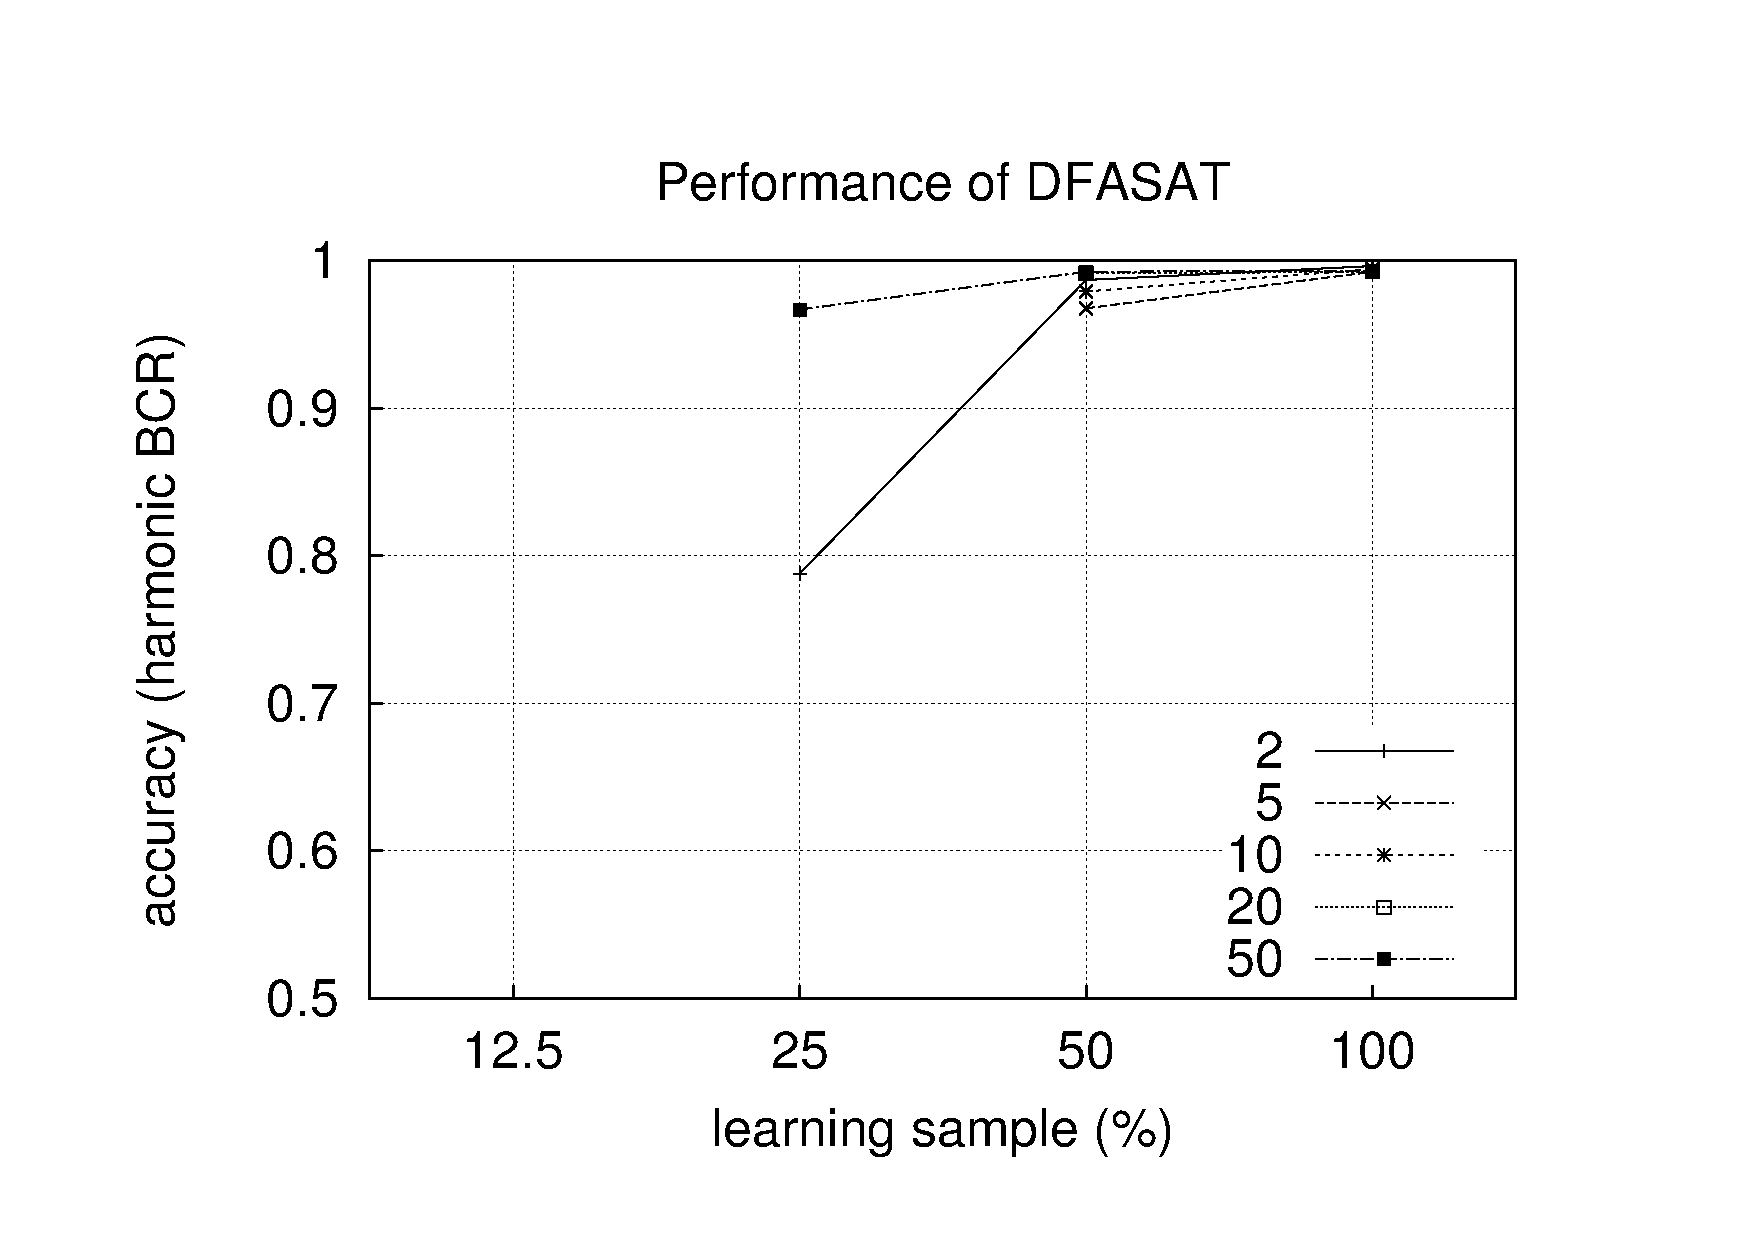
\includegraphics[trim=20mm 0mm 25mm 0mm, clip]{src/6-stamina/images/DFASAT-performance}
  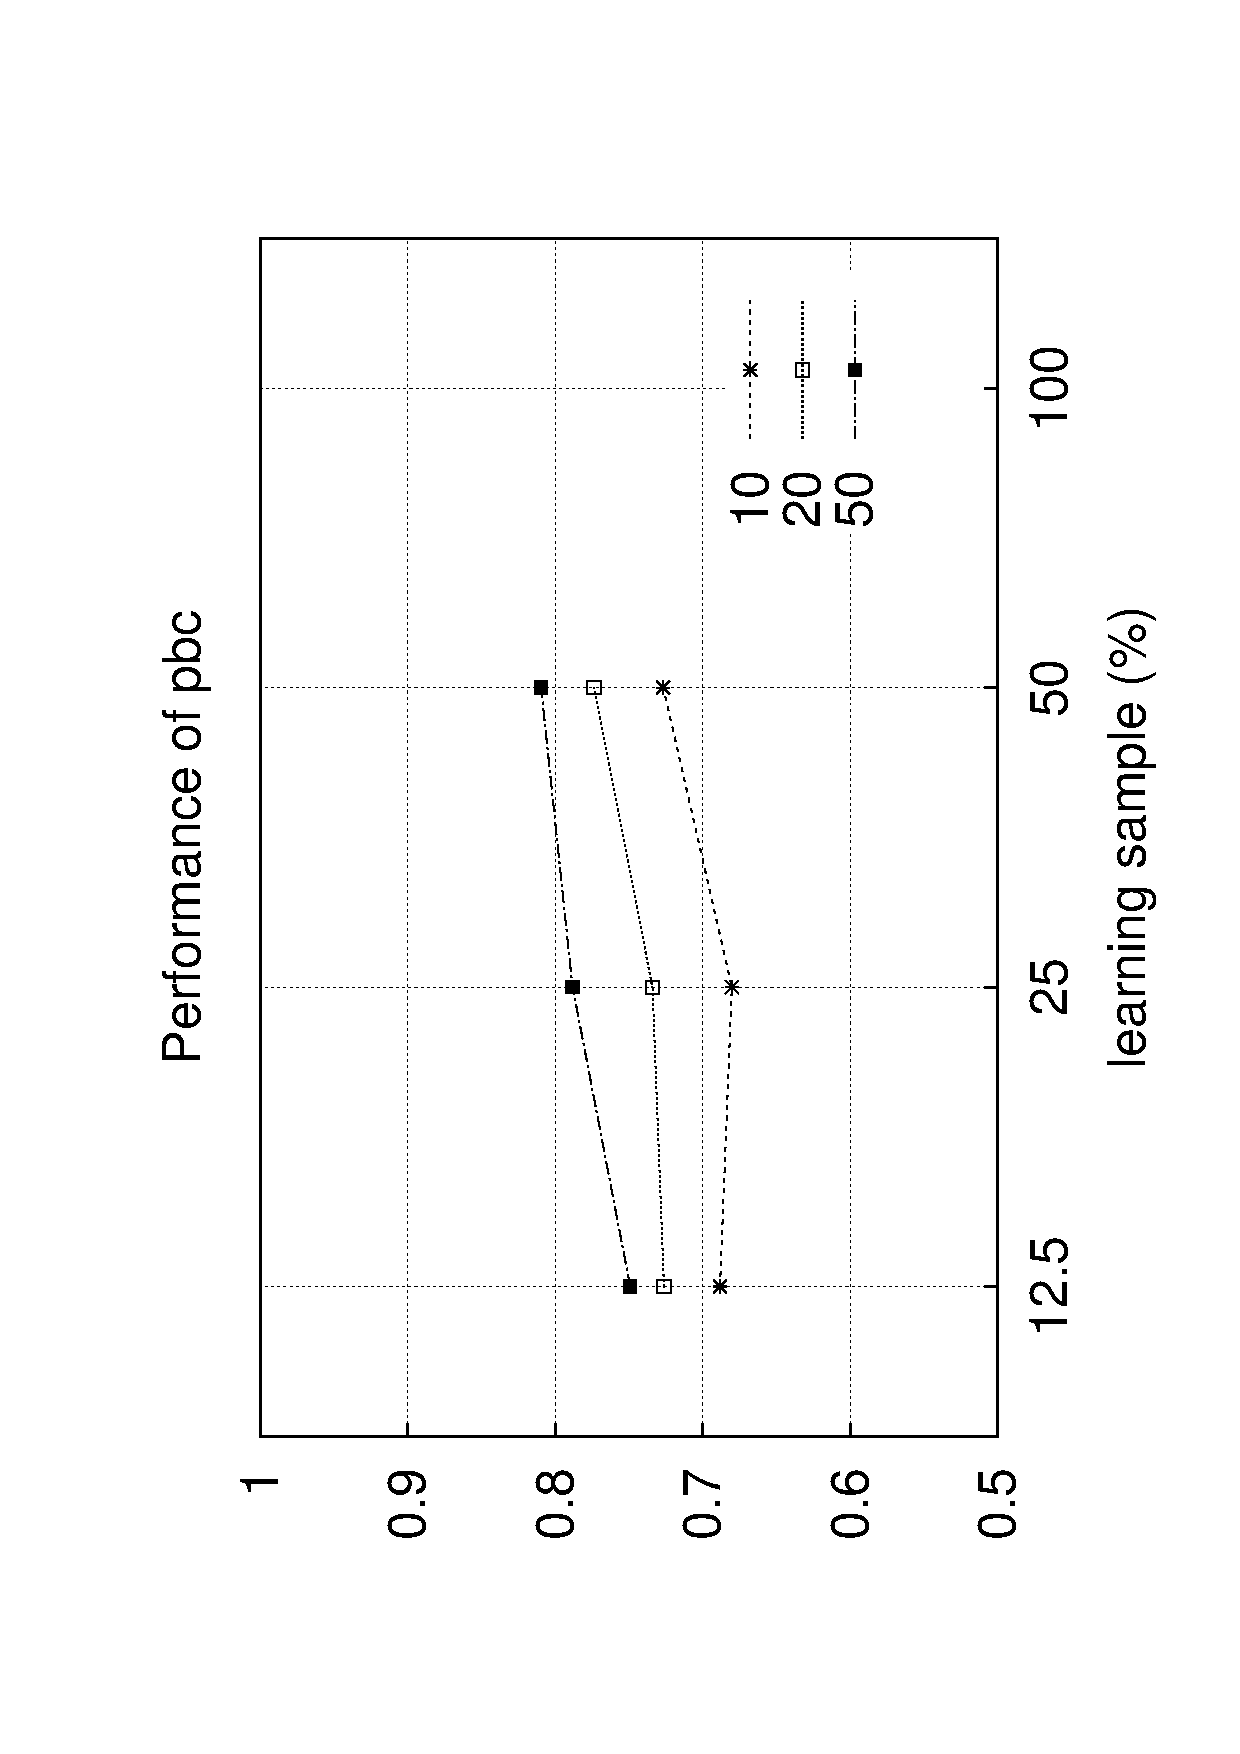
\includegraphics[trim=20mm 0mm 25mm 0mm, clip]{src/6-stamina/images/pbc-performance}}
  \caption{Performance curves of DFASAT\label{image:stamina-winners-performance-comparison}.}
\end{figure}

In any case, a quick comparison of curves from Fig.~\ref{image:stamina-winners-performance-comparison} with baseline curves given earlier in Fig.~\ref{stamina:image:bluefringe-performance} perfectly illustrates the overall contribution of the competition and of these two approaches in particular: on the kind of problems considered in Stamina, the state of the art in grammar induction has been pushed significantly forward.

%%%%%%

\section{From Stamina to an evaluation platform\label{section:stamina-platform}}

In the spirit of Abbadingo, the competition website is still available online and aims at becoming an online benchmark for evaluating novel induction techniques. To achieve this goal a few changes have already been made on the competition server:

\begin{itemize}
\item The average score obtained by Blue-fringe on each cell has been published in the documentation section of the website.
\item The public hall of fame has been updated in a direction similar to what has been discussed in Section~\ref{subsection:stamina-trends-on-hardest-cells}. Indeed, instead of displaying the winners of broken cells only, each cell is annotated with the three best challengers in descending order of their average score for that cell (which is also given). 
\item The oracle has not been modified and still gives a binary feedback only, to continue preventing hill-climbing. However, the private participant section has been updated in a similar way to the hall of fame. Now, the private submission grid displays the average score obtained on each of the cell for which she has submitted.
\item In both cases -- public hall of fame and private section -- having submitted for the five problems of a cell is a necessary condition for results to be taken into account. Imposing such a criteria guarantees sound comparisons between participants. It is also a strong incentive to run a technique on all problems of a given difficulty, overcoming the problem of having only partial results available for analyses.
\end{itemize}

These choices have been made with a double objective in mind. The first one is to provide a more transparent feedback in the form of an exact scoring mechanism helping participants to self-evaluate, without being tempted to hijack the oracle (changes in the private section). The second one is to keep a competitive aspect to the platform, which counts in the motivation for using it (implemented by the new hall of fame). 

Future work along a certain number of directions is worth considering, some of them being even required to use the plateform to evaluate the techniques of the present thesis:

\begin{itemize}

\item First, interactive inductive techniques (e.g. QSM) could hardly compete so far, due to the absence of an online oracle answering membership queries. While implementing such an oracle does not present particular difficulties (except, maybe, to guarantee scalability in presence of numerous demanding challengers), it would require generating fresh new problems to avoid interfering with the current grid and challengers already competing on it. 

\item White box benchmarks -- where target machines would be disclosed together with samples -- could also be envisaged in order to help evaluating, on a common basis, inductive techniques involving domain information 'ala' fluents or mandatory merge constraints. Alternatively, sharing binaries for generating new target machines and samples could help reusing the Stamina protocol. 

\item Last, the protocol used to generate samples (random walks from the machine, noisy perturbation to obtain negative strings and the presence of duplicates in the training set) is an interresting aspect of Stamina, that does not seem to have been used by participants. While it allows tackling the induction problem with statistical approaches, it also triggers questions about the splitting between training and test samples and the impact it could have on the observed frequency of use, in the training set, of each transition of the target. At the time of writing, further study of competition data is still required to answer the question.

\end{itemize}
